%template1.tex
%The following LaTeX source file represents the simplest kind of slide presentation; no overlays, no included graphics. Substitute your favorite style for ``pascal''. To create the PDF file template1.pdf, (1) be sure to use the prosper class, then (2) execute the command latex template1.tex, and (3) the command dvipdf template1.dvi.

%%%%%%%%%%%%%%%%%%%%%%%%%%%%%%% template1.tex %%%%%%%%%%%%%%%%%%%%%%%%%%%%%%%%%%%
\documentclass[a4paper,blends,pdf,colorBG,slideColor]{prosper}
% definitions for slides for CSC544
% Lutz Hamel, (c) 2007

\hypersetup{pdfpagemode=FullScreen}

\usepackage{times}
\usepackage{latexsym}
\usepackage{alltt}
\usepackage{booktabs}
\usepackage{amsmath}
\usepackage{amsopn}
\usepackage{amsfonts}
\usepackage{amssymb}
%\usepackage[usenames]{color}

\def\sign{\qopname\relax{no}{sign}}
\def\argmax{\qopname\relax{no}{argmax}}
\def\argmin{\qopname\relax{no}{argmin}}

\newcommand{\grad}{\ensuremath{\nabla}} 
\newcommand{\loss}{\ensuremath{{\cal L}}}
\newcommand{\err}{\mbox{err}}
\newcommand{\mse}{\mbox{mse}}
\newcommand{\acc}{\mbox{acc}}
\newcommand{\Integer}{\ensuremath{\mathbb{N}}}
\newcommand{\size}[1]{{|{#1}|}}
\newcommand{\Rnspace}[1]{\ensuremath{\mathbb{R}^{#1}}}
\newcommand{\Real}{\ensuremath{\mathbb{R}}}
\newcommand{\mytt}[1]{{\small\tt{#1}}}
\newcommand{\textemph}[1]{{\em #1}}
\newcommand{\suchthat}{\mid}
\newcommand{\orbar}{\;|\;}
\newcommand{\bs}[1]{\begin{slide}{#1}\ptsize{8}}
\newcommand{\es}{\end{slide}}
\newcommand{\co}{\,\colon\;}
\newcommand{\pair}[2]{\ensuremath{( {#1}, {#2} )}}
\newcommand{\model}[1]{\hat{#1}}
\newcommand{\ul}[1]{{\bf\em #1}}
\newcommand{\ol}{\overline}
\newcommand{\definition}[1]{{\bf Definition: }{\em #1}}
\newcommand{\example}[1]{{\bf Example: }{#1}}
\newcommand{\abs}[1]{|{#1}|}
\newcommand{\mytab}{\makebox[.1in]{}}

\newcommand{\fdef}[1]{
\begin{center}
\fbox{
\begin{minipage}{3.5in}
{\bf Definition:}
{#1}
\end{minipage}
}
\end{center}
}

\newcommand{\fframe}[1]{
\begin{center}
\fbox{
\begin{minipage}{3.5in}
{#1}
\end{minipage}
}
\end{center}
}

\newcommand{\nframe}[1]{
\begin{center}
\begin{minipage}{3.5in}
{#1}
\end{minipage}
\end{center}
}

\newenvironment{Rcode}
	{
		\scriptsize
		\begin{quote}
		\begin{alltt}
	}
	{
		\end{alltt}
		\end{quote}
	}




\begin{document}

\bs{Support Vector Machines}
\begin{itemize}
\item Support vector machines can be viewed as the {\em dual} to maximum margin classifiers.
\item Maximum margin classifiers represent optimization problems with the maximum margin
between the supporting hyperplanes as the optimization criterion.
\item A particularly convenient technique to derive the dual of an optimization problem is a
technique referred as the {\em Lagrangian dual}.
\end{itemize}
\es

\bs{Lagrangian Optimization}
\small
Assume that we have a {\em primal} optimization problem of the form,
\begin{align*}
\min_{\ol{x}} \phi(\ol{x}), \\
\intertext{such that}
g_i(\ol{x}) \ge 0,
\end{align*}
for all $\ol{x}\in \Rnspace{n}$ with $i = 1,\ldots,l$.  
Here we assume that $\phi$ is a convex objective function and we also assume that
the constraints $g_i$ are linear.

We can construct the {\em Lagrangian optimization problem} as follows,
\begin{align*}
\max_{\ol{\alpha}} \min_{\ol{x}} L(\ol{\alpha},\ol{x})& = \max_{\ol{\alpha}} \min_{\ol{x}}\left( \phi(\ol{x}) - \sum_{i=1}^l \alpha_i g_i(\ol{x})\right ),\\
\intertext{such that}
\alpha_i &\ge 0,
\end{align*}
for  $i = 1,\ldots,l$ and $\ol{x}\in \Rnspace{n}$.  
\es

\bs{Lagrangian Optimization}
Observations:
\begin{itemize}
\item The new objective function $L(\ol{\alpha},\ol{x})$ is called
the \textemph{Lagrangian} and  incorporates the original objective function
$\phi$ together with a linear combination of the constraints $g_i$.
\item The values $\alpha_1,\ldots,\alpha_l$ are called the {\em Lagrangian multipliers}.
\item We call $\ol{x}$ the {\em primal   variable} and $\ol{\alpha}$ the
{\em dual variable}.
\item This newly derived optimization problem has the unusual feature of two nested optimization operators with opposing optimization objectives.
\end{itemize}
\es

\bs{Lagrangian Optimization}
We have
\begin{align*}
\max_{\ol{\alpha}} \min_{\ol{x}} L(\ol{\alpha},\ol{x})& = \max_{\ol{\alpha}} \min_{\ol{x}}\left( \phi(\ol{x}) - \sum_{i=1}^l \alpha_i g_i(\ol{x})\right ),\\
\intertext{now let $\ol{x} = \ol{x}^*$ be an optimum then}
\max_{\ol{\alpha}} L(\ol{\alpha},\ol{x}^*) &= \max_{\ol{\alpha}} \left( \phi(\ol{x}^*) - \sum_{i=1}^l \alpha_i g_i(\ol{x}^*)\right ),\\
\intertext{now let $\ol{\alpha} = \ol{\alpha}^*$ be an optimum then}
\min_{\ol{x}} L(\ol{\alpha}^*,\ol{x}) &= \min_{\ol{x}} \left( \phi(\ol{x}) - \sum_{i=1}^l \alpha_i^* g_i(\ol{x})\right ) .
\end{align*}

\vspace{.2in}
This implies that our solutions are
\textemph{saddle points} on the graph of the function $L(\ol{\alpha},\ol{x})$. 

\es

\bs{Saddle Point}

\vspace{.2in}

\begin{center}
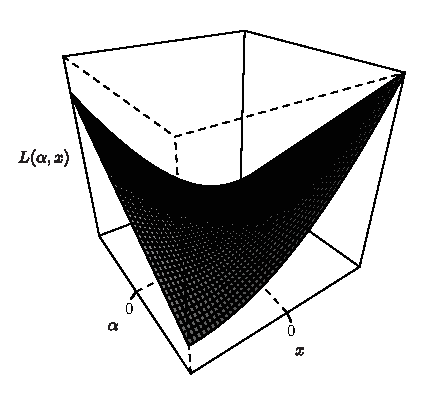
\includegraphics[height=60mm]{figures/fig07-02.eps}
\end{center}
\es


\bs{Lagrangian Optimization}
An important observation is that at the saddle point the identity
\begin{equation*}
\frac{\partial L}{\partial \ol{x}} = \ol{0},
\end{equation*}
has to hold.

This gives us the important identity
\begin{equation*}
\frac{\partial L}{\partial \ol{x}} (\ol{\alpha},\ol{x}^*)= \ol{0}.
\end{equation*}
Here, the point $\ol{x}^*$ represents an optimum of $L$ with respect to $\ol{x}$.
\es

\bs{Lagrangian Optimization}
\small
This allows us to formulate our first major result in Lagrangian optimization theory.
Let $\ol{\alpha}^*$ and $\ol{x}^*$ be a solution to
the Lagrangian such that,
\begin{equation*}
\max_{\ol{\alpha}} \min_{\ol{x}} L(\ol{\alpha},\ol{x}) = L(\ol{\alpha}^*,\ol{x}^*)
	=  \phi(\ol{x}^*) - \sum_{i=1}^l \alpha^*_i g_i(\ol{x}^*),
\end{equation*}
then $\ol{x}^*$ is a solution to the primal
objective function if and only if the following conditions hold,
\begin{align*}
\frac{\partial L}{\partial \ol{x}}(\ol{\alpha}^*, \ol{x}^*) &= \ol{0},\\
\alpha^*_i g_i(\ol{x}^*) &= 0,\\
g_i(\ol{x}^*) &\ge 0,\\
\alpha_i^* &\ge 0,
\end{align*}
for $i = 1,\ldots,l$.

These conditions are collectively referred to as the \textemph{Karush-Kuhn-Tucker (KKT) conditions}
and if satisfied ensure that
\begin{equation*}
L(\ol{\alpha}^*,\ol{x}^*) =  \phi(\ol{x}^*). \text{   (Why?)}
\end{equation*}

{\bf NOTE:} The KKT conditions are always satisfied for convex optimization problems!
 
\es

\bs{Lagrangian Dual}
\small
Now let $\ol{x}^*$ be an optimum, that is,
\begin{equation*}
\frac{\partial L}{\partial \ol{x}} (\ol{\alpha},\ol{x}^*)= \ol{0},
\end{equation*}
then we can rewrite our Lagrangian as an objective function of only the dual variable,
\begin{equation*}
L(\ol{\alpha}, \ol{x}^*) = \phi'(\ol{\alpha}).
\end{equation*}
We call the function $\phi'$ the \textemph{Lagrangian dual}.

This gives us our new, dual optimization problem
\begin{align*}
 \max_{\ol{\alpha}} \phi'(\ol{\alpha}),\\
 \intertext{subject to}
 \alpha_i \ge 0,
\end{align*}
for $i = 1,\ldots,l$.

\begin{quote}
{\bf NOTE:} Observe that
\begin{equation*}
\max_{\ol{\alpha}} \phi'(\ol{\alpha}) = \phi'(\ol{\alpha}^*) = L(\ol{\alpha}^*,\ol{x}^*) =  \phi(\ol{x}^*),
\end{equation*}
if the KKT conditions are satisfied.
\end{quote}

\es


\bs{An Example}
\small
Consider the convex optimization problem, 
\begin{align*}
\min \phi(x) &= \min \frac{1}{2} x^2,\\
\intertext{subject to the linear constraint}
g(x)& = x - 2 \ge 0,
\end{align*}
with $x \in \Real$.

\begin{center}
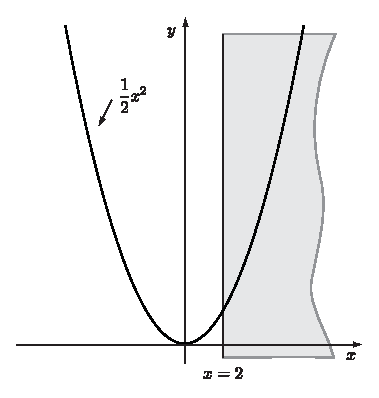
\includegraphics[height=40mm]{figures/fig07-01.eps}
\end{center}
\es


\bs{An Example}
In order to solve this optimization problem using the Lagrangian dual we first construct the Lagrangian,
\begin{equation*}
\label{eq:simple-lagranian-opt}
L(\alpha,x)  = \frac{1}{2}x^2 - \alpha(x - 2).
\end{equation*}

As expected for a convex objective function we have a unique saddle point in the graph of the Lagrangian,  

\begin{center}
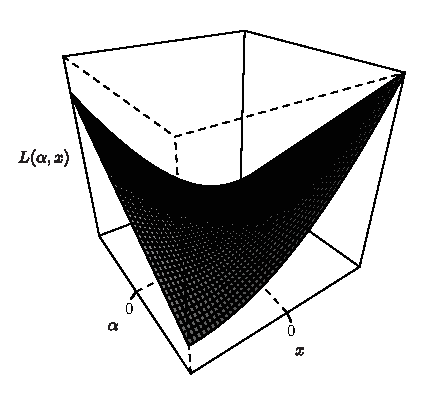
\includegraphics[height=40mm]{figures/fig07-02.eps}
\end{center}
\es

\bs{An Example}
\small
We know that this saddle point has to occur where the gradient of the Lagrangian with
respect to the variable $x$ is equal to zero, 
\begin{equation*}
\frac{\partial L}{\partial x} (\alpha, x^*)=  x^* - \alpha = 0.
\end{equation*}
Solving for $x^*$ gives us,
\begin{equation*}
 x^* = \alpha.
\end{equation*}
Now, plugging this identity back into the Lagrangian
gives us,
\begin{equation*}
L(\alpha,x^*) = \frac{1}{2}\alpha^2 - \alpha^2 + 2\alpha = 2\alpha - \frac{1}{2}\alpha^2.
\end{equation*}
This Lagrangian has no longer any dependencies on the variable $x$ and therefore
we can rewrite this as the Lagrangian dual with $\phi'(\alpha) = L(\alpha,x^*)$ or,
\begin{align*}
\max_{\alpha} \phi'(\alpha)& = \max_{\alpha} \left(2\alpha - \frac{1}{2}\alpha^2 \right )
\\
\intertext{subject to}
\alpha &\ge 0.
\end{align*}

\es

\bs{An Example}
Now we know that $L(\alpha,x)$ is convex, therefore $\phi'(\alpha^*) = \max_\alpha \phi'(\alpha)$
implies that
\begin{equation*}
\frac{d\phi'}{d\alpha}(\alpha^*)= 2 - \alpha^*= 0.
\end{equation*}
This means that,
\begin{equation*}
x^* = \alpha^* = 2,
\end{equation*}
as required by our observation of the primal optimization problem.

Formally we can show that the solution to the primal optimization problem and to the Lagrangian dual
must 
coincide by showing that that the second KKT condition is satisfied,
\begin{equation*}
\alpha^*g(x^*) = \alpha^*(x^* - 2) = 2(2-2) = 0.
\end{equation*}

\es

\end{document}
%%%%%%%%%%%%%%%%%%%%%%%%%%% end of template1.tex %%%%%%%%%%%%%%%%%%%%%%%%%%%%%%%%

